\begin{frame} \frametitle{Context: smart card certification}
\vfill
% Composants sécurisés = cartes à puce : utilisées partout
% PEUVENT ÊTRE ATTAQUEES ! Par un voleur, l'utilisateur, etc...
% Sont protégées et leur sécurité est évaluée avant leur mise sur le marché
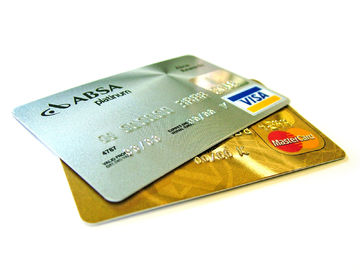
\includegraphics[height=1cm]{sm1.jpg} 
\vfill
\begin{block}{Smart cards}
\begin{itemize}
\item Pervasive : bank, health, phones, \ldots (7 billions sold in 2012) 
\vfill
\item Contain sensible data and applications 
		\alert{{\bf $\Rightarrow$ can be attacked!}}
\end{itemize}
\end{block}
\vfill
\begin{block}{Smart card security}
\begin{itemize}
	\item Protections mechanisms added by manufacturers 
	\item Well-defined \alert{certification process}, prior to commercialization:
	\begin{itemize}
		\item Security functional test
		\item \alert{Penetration test} 
	\end{itemize}
\end{itemize}
\end{block}
\begin{block}{Certification procedures include}
	\begin{itemize}
	\item Physical testing on the device (black box)
	\item \alert{Code review and/or code analysis (white box)}
	\end{itemize}
\end{block}
\vfill
\end{frame}

%\IGNORE{
%\begin{frame} \frametitle{A typical certification process}
%\vfill
%\begin{figure}
%\begin{tikzpicture}[scale=0.60,every node/.style={transform shape}] 
%    % Place nodes
%    \node [decision] (oktestsw) {Are tests OK?};
%    \node [block, left of=oktestsw] (testsw) {Try to forecast vulnerabilities};
%    \node [block, left of=testsw] (code) {Develop secure application};
%    \node [block, right of=oktestsw] (eval) {Evaluate conformity and vulnerabilities};
%    \node [decision, right of=eval] (okeval) {Is evaluation OK?};
%    \node [block, right of=okeval] (cert) {Emit certificate};
%    %actors
%    \node [cloud, below of=code] (dev) {Developer};
%    \node [cloud, below of=eval] (cesti) {ITSEF (CESTI)};
%    \node [cloud, below of=cert] (anssi) {ANSSI};
%
%        %conditions
%    % Draw edges
%    %actors -- actions
%    \path [line, dashed] (dev) -- (code);
%    \path [line, dashed] (dev) -- (testsw);
%    \path [line, dashed] (cesti) -- (eval);
%    \path [line, dashed] (anssi) -- (cert);
%    % actions -- next_actions
%    \path [line] (code) -- (testsw);
%    % actions -- decisions
%    \path [line] (eval) -- (okeval);
%    \path [line] (testsw) -- (oktestsw);
%    % decisions -- actions
%    \path [line] (oktestsw) -- +(0, 2) -| node[near start, above] {no}(code);
%    \path [line] (oktestsw) -- node[above] {yes}(eval);
%    \path [line] (okeval) -- +(0, 3) -| node[near start, above] {no}(code);
%    \path [line] (okeval) -- node[above] {yes}(cert);
%\end{tikzpicture}
%\end{figure}
%\vfill
%\pause
%$\rightarrow$ Evaluation performed according to the \alert{Common Criteria}
%\begin{itemize}
%	\item black box: physical testing on the device
%	\item white box: code review and/or code analysis 
%\end{itemize}
%\vfill
%\end{frame}
%}
%
%
%\begin{frame} \frametitle{Fault injection based attacks}
%% L'injection de faute est 1 attaque réalisée physiquement qui change l'exec
%\vfill
%$\bullet$ physical attack performed at runtime \\
%	$\quad$ $\leadsto$
%\textbf{change the data read} or  \textbf{modify the executed code} \\
%$\bullet$ several techniques: \\ $\quad$ laser/electromagnetic perturbation, clock acceleration \dots
%%A model for what happens:
%    \begin{figure}
%    \begin{tikzpicture}[remember picture,
%    scale=0.80,
%    % define styles here
%    every node/.style={transform shape}
%    ]
%    \draw[rounded corners] (0, 0) rectangle (5, 3);
%
%    \node (chip) at (0.7,2) { \usebox\chip };
%    \draw[fill=circolor] (1.4, 0.4) rectangle (4.6, 2.6);
%    \node[fill=cpucolor] (CPU) at (2.0, 1.5) [draw, thick, minimum width=1.0cm,
%    minimum height=2.0cm, font=\small] {\textbf{CPU}};
%    \node[fill=memcolor] (Mem) at (4.0, 2.25) [draw, thick, minimum width=1.0cm,
%    minimum height=0.5cm, font=\small] {\textbf{Mem}};
%    %\draw[fill=buscolor] (2.5, 1.3) rectangle (3.5, 1.7) node[font=\tiny, midway]{Bus};
%    \draw[middlearrow={<}, very thick] (CPU) -- (4.0, 1.5) -- (Mem);
%    \draw[color=attackcolor] (3.25, 1.80) -- (3.05, 1.60) --
%    (3.25, 1.40) -- (3.05, 1.20)
%        node[color=attackcolor, midway, below]{\scriptsize{attack}};
%    \node[font=\scriptsize] (valmem) at (4.3, 1.8) {0x3a};
%    \node[font=\scriptsize, color=red] (valcpu) at (2.8, 1.35) {0x42};
%    \end{tikzpicture}
%    \end{figure}
%\vfill
%% Au niveau binaire ça donne :
%\vfill
%\begin{table}
%\centering
%%% init
%\only<1>{
%\begin{tabular*}{0.99\linewidth}{|c @{\extracolsep{\fill}}||c|c|c|}
%\hline
%Instruction             & \multicolumn{3}{c|}{LD R0 M[23] ; Loads M[23]=0x72 in R0} \\
%\hline
%Memory access number    & 1         & 2         & 3 \\
%Address                 & 0xEE1223  & 0xEE1224  & 0x23 \\
%Value                   & 0x87      & 0x23      & 0x72 \\
%\hline
%\end{tabular*}
%}
%\only<2>{
%%% perturbation n°1
%\begin{tabular*}{0.99\linewidth}{|c @{\extracolsep{\fill}}||c|c|c|}
%\hline
%Instruction             & \multicolumn{3}{c|}{LD R0 23 ; Loads
%immediate 0x23 in R0} \\
%\hline
%Memory access number    & 1         & 2         & 3 \\
%Address                 & 0xEE1223  & 0xEE1224  & Discarded \\
%Value                   & \textbf{\textcolor{red}{0x42}}
%& 0x23      & Discarded \\
%\hline
%\end{tabular*}
%}
%\only<3>{
%%% perturbation n°2
%\begin{tabular*}{0.99\linewidth}{|c @{\extracolsep{\fill}}||c|c|c|}
%\hline
%Instruction             & \multicolumn{3}{c|}{LD R0 M[42] ; Loads
%M[42]=0x66 in R0} \\
%\hline
%Memory access number    & 1         & 2         & 3 \\
%Address                 & 0xEE1223  & 0xEE1224  & 0x42 \\
%Value                   & 0x87      & \textbf{\textcolor{red}{0x42}}      & 0x66 \\
%\hline
%\end{tabular*}
%}
%\only<4>{
%%% perturbation n°3
%\begin{tabular*}{0.99\linewidth}{|c @{\extracolsep{\fill}}||c|c|c|}
%\hline
%Instruction             & \multicolumn{3}{c|}{LD R0 M[23] ; Loads 0x42 in R0} \\
%\hline
%Memory access number    & 1         & 2         & 3 \\
%Address                 & 0xEE1223  & 0xEE1224  & 0x23 \\
%Value                   & 0x87      & 0x23      & \textbf{\textcolor{red}{0x42}} \\
%\hline
%\end{tabular*}
%}
%\only<1>{\caption{Initial instruction}}
%\only<2>{\caption{Opcode perturbation}}
%\only<3>{\caption{Operand perturbation}}
%\only<4>{\caption{Data perturbation}}
%\end{table}
%\vfill
%\end{frame}

\begin{frame}[fragile] \frametitle{Effects of fault injection at the source level}
% Au niveau source ça peut se traduire par :
\begin{columns}[t]
\begin{column}{0.50\textwidth}
\begin{lstlisting}[
  basicstyle=\footnotesize\ttfamily,
]
int verify(char buffer[4]) 
{
  int i;
  for(i = 0; i < 4; i++)
    if(buffer[i] != pin[i]) {
      authenticated = 0;
      goto FAILURE;
    }
  authenticated = 1;
  return EXIT_SUCCESS;
  FAILURE : return EXIT_FAILURE;
}
\end{lstlisting}
\end{column}
\begin{column}{0.48\textwidth}
\begin{lstlisting}[style=customasm,
%\begin{lstlisting}[language={[x86masm]Assembler},
  basicstyle=\footnotesize\ttfamily,
]
MOV R3, #01h 
MOV R0, #00h
WHILE: MOV A, R0
SUBB A, #04h
JZ END // exit loop
DO:
MOV R2, [buffer+i] 
MOV A, [pin+i] 
SUBB A, R2 
JZ SUCCESS 
MOV R3, #00h
JMP END

SUCCESS: INC R0
JMP WHILE

END: MOV authenticated, R3
RET
\end{lstlisting}

\end{column}
\end{columns}
\end{frame}

%\begin{frame} \frametitle{Code-level protections against fault injections}
%\vfill
%% Problème : la combinatoire des injection
%\begin{block}
%{State of the art in fault injection attacks}
%\begin{itemize}
%\item volatile faults, occuring at run-time ($\neq$ code modification)
%\item multiple spatial and/or temporal faults (up to 2)
%\end{itemize}
%\begin{center}
%\fbox{
%	\alert{$\rightarrow$  
%		impossible to check all fault combinations in practice \dots}
%}
%\end{center}
%\end{block}
%\vfill
%\pause
%\begin{block}
%{Code-level counter-measures}
%\begin{itemize}
%\item instruction counters, check call/exit procedure consistency
%\item duplicated evaluation of conditional expressions
%\item duplicated procedure execution
%\item split/replicate information in several memory locations 
%\item etc.
%\end{itemize}
%\begin{center}
%\fbox{\alert{Are these counter-measures useful ? sufficient ?}}
%\end{center}
%\end{block}
%\vfill
%\end{frame}
%
%\begin{frame}[fragile] \frametitle{Counter-measure examples}
%\begin{lstlisting}[
%  basicstyle=\scriptsize\ttfamily,
%  commentstyle=\color{red}
%]
%int stepCounter = INITIAL_VALUE ; // Instruction counter
%
%int verify(char buffer[4]) {
%  int i;
%  for(i = 0; i < 4; i++) {
%    if(buffer[i] == pin[i]) {
%       if(buffer[i] != pin[i]) {  // Duplicated test
%          authenticated = 0;
%          goto FAILURE;
%       } else {
%          authenticated = 0;
%          goto FAILURE;
%       } ;
%       stepCounter ++ ; // Increment the inst. counter
%    } ;
%  if (stepCounter == INITIAL_VALUE + 4) { 
%     authenticated = 1;
%     return EXIT_SUCCESS; // Each pin byte double checked
%  } else {
%     authenticated = 0 ;
%     goto FAILURE ;
%  } ;
%FAILURE : return EXIT_FAILURE;  // Card is lost ...
%}
%\end{lstlisting}
%
%\end{frame}


%\begin{frame} \frametitle{Work Objective: Developer/Auditor point of view}
%\vfill
%\begin{block}
%{$\rightarrow$ Assist the robustness evaluation against fault injection}
%\vfill
%\begin{itemize}
%\item White box evaluation as a source-level code analysis
%\item Handle state-of-the-art attacks: multiple volatile faults  
%\end{itemize}
%\end{block}
%\vfill
%$\rightarrow$ To be completed with more specific analysis, simulation, physical testing, etc.
%\vfill
%\end{frame}

\begin{frame} \frametitle{Security Property and Fault Model}
\vfill
\begin{block}{Security Property}
\begin{center}
$\hookrightarrow$ \alert{Enforce} or \alert{prevent} the execution of specific instruction(s).
\alert{$\Rightarrow$ Attack Objective = set of basic blocks (not) to be reached} 
\end{center}
\end{block}
\vfill
\begin{block}
{Objectives of the analysis:} 
\begin{itemize}
\item \alert{Predict} (or \alert{prove the absence of}) possible attacks,
		for a given fault model
\item \alert{Locate} the ``dangerous spots'' in the code 
\item \alert{Evaluate} the relevance of existing counter-measures 
\end{itemize}
\end{block}
\vfill
\begin{block}{Fault Model - Multiple faults}
Volatile control structure \alert{test inversion} (e.g., {\tt if}, {\tt while}, etc.) \\
$\hookrightarrow$ Encompass multiple binary-level attacks, e.g.,
\begin{itemize} 
\item NOP injection, modify flag or register value, \dots
\end{itemize} 
\end{block}
\vfill
\end{frame}







